    Vamos a calcular las masas efectivas en función de las movilidades y las vidas medias:

    \begin{equation}
        \mu_n = D_n \frac{q}{kT} = \frac{q}{kT} \tau_n v^2_{th} = \frac{q}{kT} \tau_n \frac{3kT}{m_n^*} = \frac{3q\tau_n}{m_n^*}
    \end{equation}
    Entonces:
    \begin{equation}
        m_n^* = \frac{3q\tau_n}{\mu_n} \qquad m_p^* = \frac{3q\tau_p}{\mu_p^*}
    \end{equation}
    Usando estas ecuacioens obtenemos:

    \begin{equation}
        m_p^* = 3.88 \cdot 10^6 \ m_e \tquad m_n^* = 11.5 \cdot 10^6 \ m_e
    \end{equation}
    Francamente no se que puede estar mal, pero usaremos las masas típicas $m_p^* = 0.81m_e$ y $m_n=1.18 m_e$.
    \begin{enumerate}[label=\alph*)]
        \item Tenemos que calcular la anchura de todas las regiones del dispositivo y las bandas de energía (banda de conducción, banda de valencia, nivel de Fermi y nivel de Fermi intrínseco). También tenemos que calcular las distancias relativas entre los niveles (lo cual es obvio dado lo anterior).

        Primero tenemos que calcular las distancias, lo cual es simplemente aplicar las fórmulas para la situación de equilibrio
        \begin{equation}
            x_p = \ccorchetes{\frac{2K_S\varepsilon_0}{q} \frac{N_D}{N_A(N_A+N_D)}  V_{bi}}   \qquad
            x_n = \ccorchetes{\frac{2K_S\varepsilon_0}{q} \frac{N_A}{N_D(N_A+N_D)}  V_{bi}}
        \end{equation}
        Así pues, los valores numéricos son:

        \begin{equation}
            x_p = 5.000\cdot 10^{-5}  \ [\cm] \qquad x_n =1.000\cdot 10^{-4}  \ [\cm] \qquad W = x_n + x_p = 1.5 \cdot 10^{-4} \ [\cm ]
        \end{equation}
        Y luego tenemos que calcular los valores de todas y cada una de las bandas. Para conocer las banda, teniendo en cuenta que $E_F=0 \ [\eV]$  \textit{a lo largo de todo el dispositivo pn}. Por el resto simplemente aplicar las ecuaciones de la sección 2, tal que en la zona $p$ los valores son los que típicamente esperaríamos para un semiconductor $N_A$, mientras que en la zona $n$ será los que esperaríamos en un conductor $N_A$ menos $V_{bi}$. En la \textit{zona de vaciamiento} los valores de las bandas simplemente valdrán su valor en $p$ menos el valor $V(x)$:
        \begin{equation*}
            V_{bi} = \frac{kT}{q} \ln \parentesis{\frac{N_AN_D}{n_i^2}} = 0.580 \ [\unit{V}]
        \end{equation*}
        \begin{equation*}
            V(x) = \left\lbrace \begin{array}{ll}
                - \frac{qN_A}{2K_S\varepsilon_0} \parentesis{x_p + x}^2  & \ - x_p \leq x \leq 0 \\
                - \frac{qN_D}{2K_S\varepsilon_0} \parentesis{x_n - x}^2 + V_{bi}  & \ 0 \leq x \leq x_n \\
            \end{array} \right.
        \end{equation*}
        Por el resto de situaciones, tenemos que en la zona $p$ las ecuaciones son:
        \begin{equation*}
            E_i = - kT \ln \parentesis{\frac{n}{n_i}} = kT \ln \parentesis{\frac{N_A}{n_i}} \qquad E_c  = E_i  + kT \ln \parentesis{\frac{N_c}{n_i} } \qquad E_v  =E_c-E_g
        \end{equation*}
        tal que
        \begin{equation*}
            E_g = 1.12 \ [\eV] \qquad N_C = 2 \parentesis{\frac{m_n^* kT}{2\pi \hbar^2}}^{3/2}  = 3.21 \cdot 10^{19} \ [\cm^{-3}] \end{equation*}
        \begin{equation*}
           N_V = 2 \parentesis{\frac{m_p^* kT}{2\pi \hbar^2}}^{3/2} = 1.83 \cdot 10^{19} \ [\cm^{-3}]
        \end{equation*}
        \begin{equation*}
            n_i = \sqrt{N_CN_V} e^{-E_g/kT} = 9.49 \cdot 10^9 \ [\cm^{-3}]
        \end{equation*}
        Así pues obtenemos los siguientes resultados numéricos:
        \begin{center}
            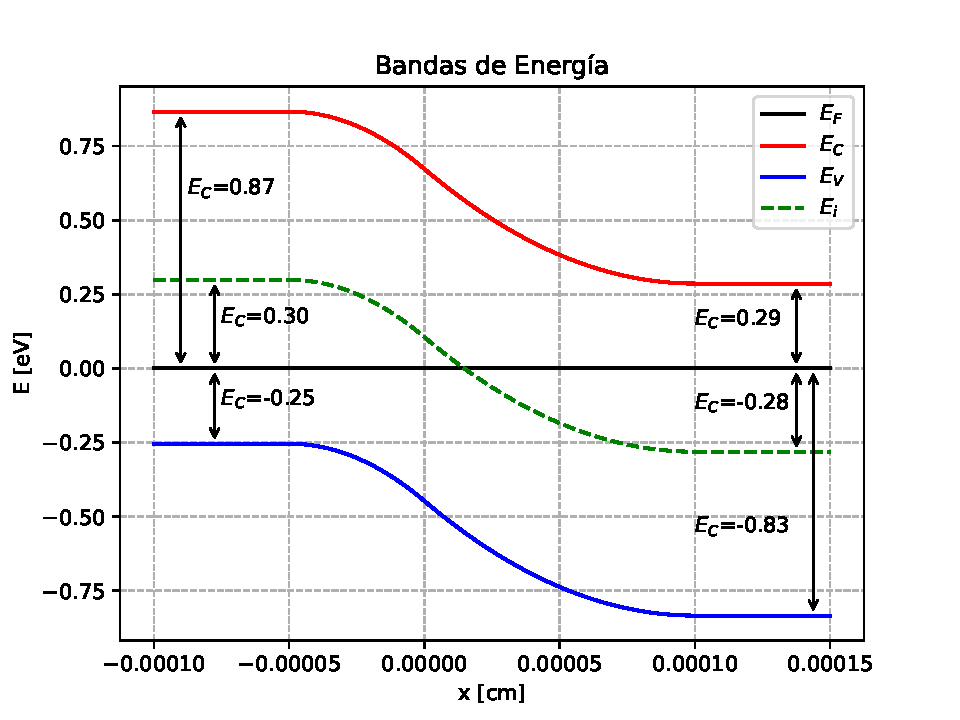
\includegraphics[width=0.6\linewidth]{Cuerpo/Ch_03/03_01_Bandas.pdf}
        \end{center}
        \item Si polarizamos la zona N con 0.2 voltios ($V_A=-0.2$V) estamos en el régimen de polarización inversa. El calculo de los anteriores valores es exáctamente igual solo que ahora tenemos que $V_{bi}\rightarrow V_{bi}-V_A$. Así pues:
        \begin{equation}
            x_p = 5.79867 \cdot 10^{-5}  \ [\cm ] \tquad
            x_n = 1.15973 \cdot 10^{-4}  \ [\cm ]
        \end{equation}xp=[cm]
        \begin{center}
            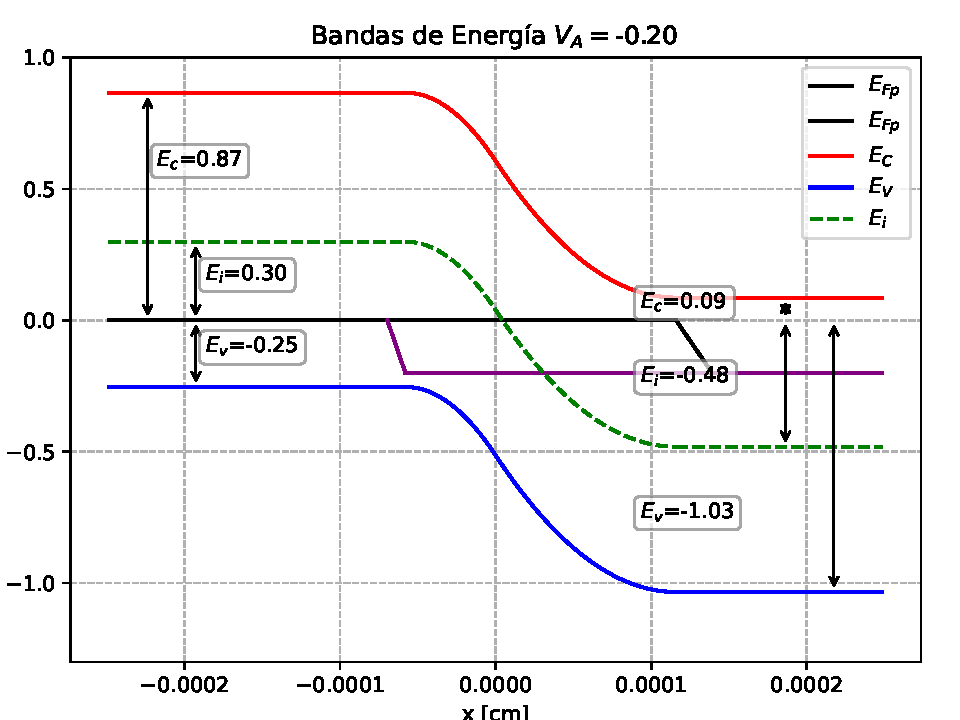
\includegraphics[width=0.6\linewidth]{Cuerpo/Ch_03/03_02_Bandas.pdf}
        \end{center}

        \item Si polarizamos la zona P con 0.2 voltios ($V_A=0.2$V) estamos en el régimen de polarización directa. El calculo de los anteriores valores es exáctamente igual solo que ahora tenemos que $V_{bi}\rightarrow V_{bi}-V_A$. Así pues:
        \begin{equation}
            x_n =8.09502 \cdot 10^{-5}  \ [\cm ] \tquad x_p = 4.04751 \cdot 10^{-5}  \ [\cm ]
        \end{equation}
        \begin{center}
            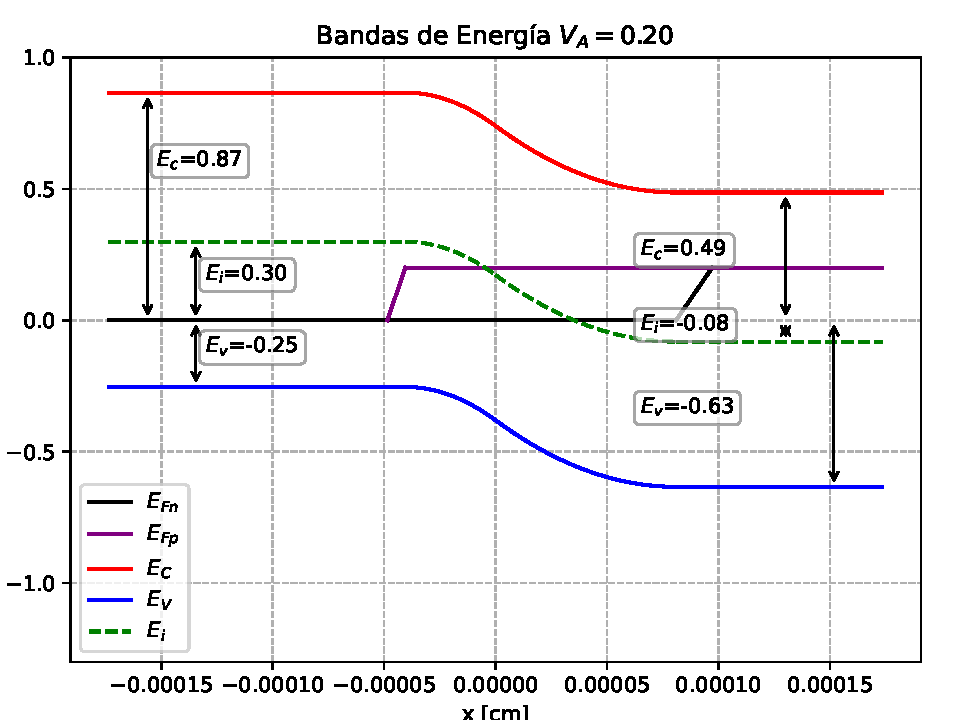
\includegraphics[width=0.6\linewidth]{Cuerpo/Ch_03/03_03_Bandas.pdf}
        \end{center}
        Ahora nos piden calcular el campo eléctrico, la densidad de carga y el voltaje a lo largo del dispositivo, así como las corrientes a lo largo del mismo. Para calcular el campo eléctrico tenemos que usar la típica fórmula:

        \begin{equation}
            \Ecal = - \derivadas{V}{x} = \frac{1}{q} \derivadas{E_i}{x}
        \end{equation}
        Así por lo tanto tenemos que:

        \begin{equation*}
            \Ecal(x) = \left\lbrace \begin{array}{ll}
                 \frac{qN_A}{K_S\varepsilon_0} \parentesis{x_p - x}  & \ - x_p \leq x \leq 0 \\
                - \frac{qN_D}{K_S\varepsilon_0} \parentesis{x_n - x} & \ 0 \leq x \leq x_n \\
            \end{array} \right.
        \end{equation*}
        siendo 0 en el resto de puntos del dispositvo. El volaje se calcula teniendo en cuenta la anterior ecuación (considerando que el cero del potencial está en la zona $p$) on la ecuación que hemos usado previamente (a). Solo falta calcular la densidad de carga, que se hace usando, por ejemplo, la ecuación de Maxwell

        \begin{equation}
            \nabla \cdot E = \frac{\rho}{K_S \varepsilon_0}
        \end{equation}
        de tal modo que:

        \begin{equation}
            \rho (x) = \left\lbrace \begin{array}{ll}
                - q N_A   & \ - x_p \leq x \leq 0 \\
                q N_D \parentesis{x_n - x} & \ 0 \leq x \leq x_n \\
            \end{array} \right.
        \end{equation}
        Lo cual es en realidad trivial o directo, ya que procede de las hipótesis de vaciamiento que usamos para deducir todas las ecuaciones (en las condiciones que exigimos para la verificación de todas estas ecuaciones incluye que $n_n,p_p\ll N_D,N_A$) de tal modo que la ecuación de la carga es la primera condición, no la última. En cualquier caso, hacemos las representaciones gráficas:
        \begin{center}
            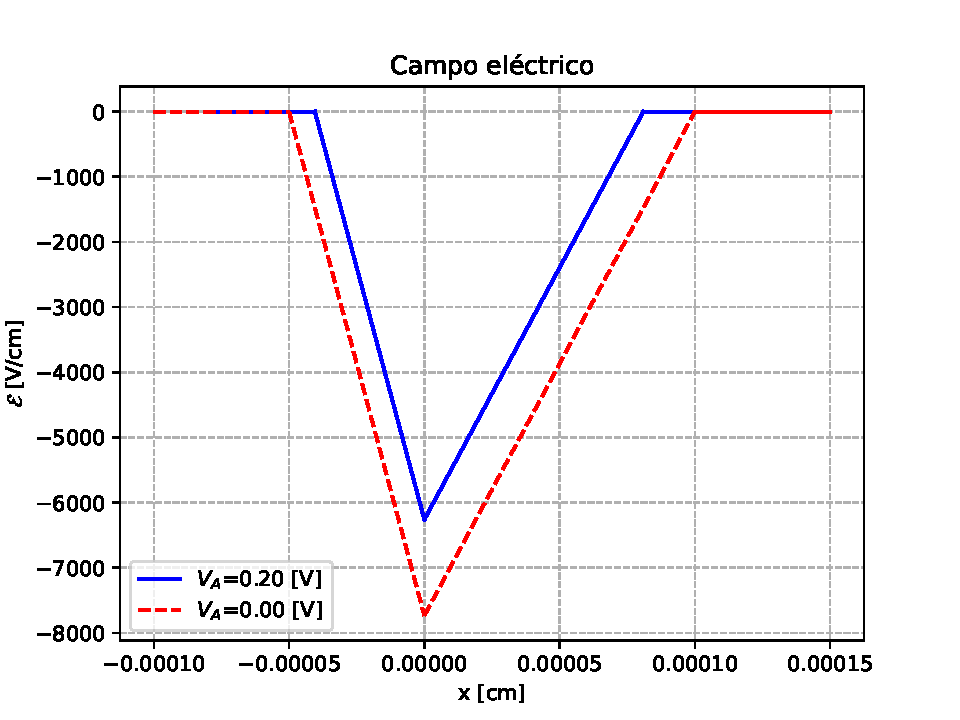
\includegraphics[width=0.6\linewidth]{Cuerpo/Ch_03/03_04_E.pdf}
        \end{center}
        \begin{center}
            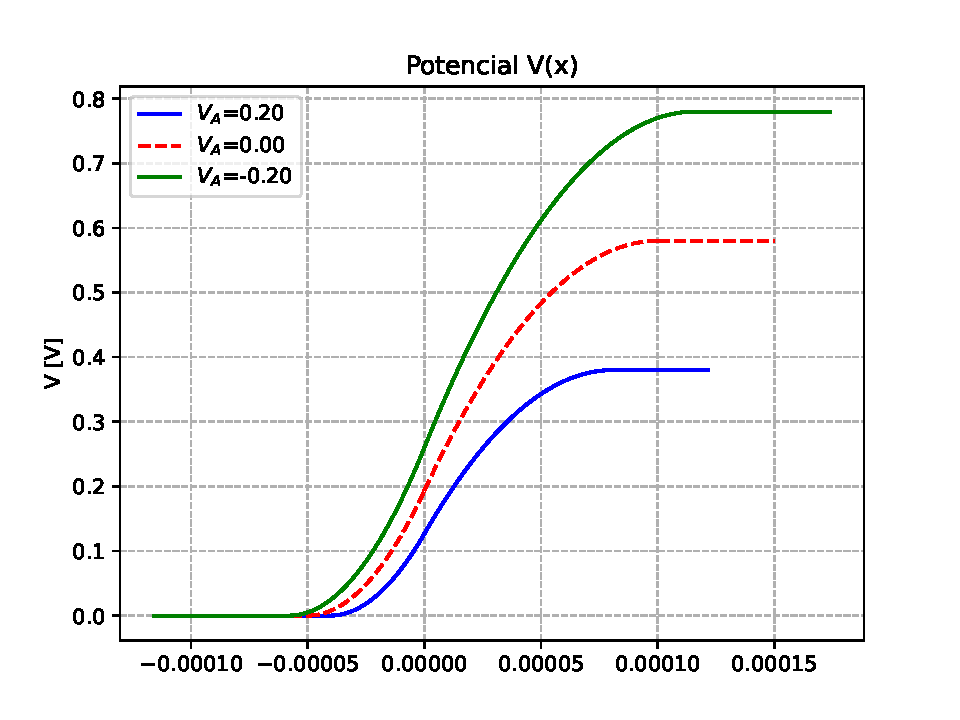
\includegraphics[width=0.6\linewidth]{Cuerpo/Ch_03/03_05_V.pdf}
        \end{center}
        \begin{center}
            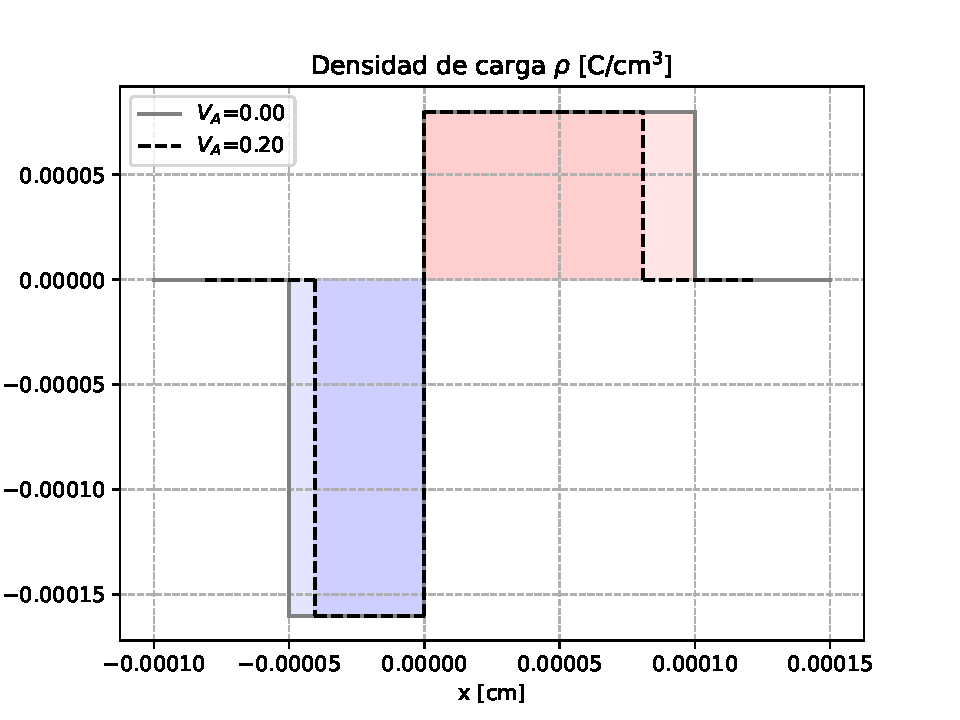
\includegraphics[width=0.6\linewidth]{Cuerpo/Ch_03/03_06_rho.pdf}
        \end{center}
        Ahora tenemos que calcular las corrientes a lo largo del dispostivo. Las corrientes
    \end{enumerate}
